%!TEX root = ../template.tex
%%%%%%%%%%%%%%%%%%%%%%%%%%%%%%%%%%%%%%%%%%%%%%%%%%%%%%%%%%%%%%%%%%%%
%% chapter10.tex
%% NOVA thesis document file
%%
%% Chapter with lots of dummy text
%%%%%%%%%%%%%%%%%%%%%%%%%%%%%%%%%%%%%%%%%%%%%%%%%%%%%%%%%%%%%%%%%%%%

\typeout{NT FILE chapter10.tex}%

\chapter{Figures, Tables, and Illustrations}
\label{chap:floats}

\section{Overview}

Figures, tables, and other illustrations play a central role in academic writing.  
\gls{novathesis} provides a coherent framework for managing these visual elements while preserving typographic consistency, institutional compliance, and full cross-referencing capabilities.

This chapter describes how to include, format, and reference figures and tables in \gls{novathesis}, as well as how to control float placement, numbering, and captioning.  
It also covers best practices for image quality, reproducibility, and accessibility.

\section{Float Management in \LaTeX}

\gls{novathesis} inherits its float management from the \texttt{memoir} class, which extends the standard \LaTeX{} float system.  
Floats are environments that contain non-text elements (figures, tables, algorithms, etc.) that can move to the most suitable position in the layout.

Common environments include:
\begin{quote}
\texttt{figure}, \texttt{table}, \texttt{sidewaysfigure}, and \texttt{longtable}.
\end{quote}

Each float consists of three key components:
\begin{itemize}
  \item the content (e.g., an image or tabular data);
  \item a caption (\verb|\caption{...}|);
  \item an internal label (\verb|\label{...}|) for referencing.
\end{itemize}

\section{Including Figures}
\label{sec:figures}

Figures are stored in the directory \texttt{5-Figures/}.  
Supported formats include \texttt{.pdf}, \texttt{.png}, and \texttt{.jpg}.  
Vector formats (\texttt{.pdf} or \texttt{.eps}) are recommended for line art and diagrams; raster formats (\texttt{.png}) are preferred for screenshots or photographs.

\paragraph{Basic Example.}
\begin{verbatim}
\begin{figure}[htbp]
  \centering
  \includegraphics[width=0.75\linewidth]{5-Figures/example}
  \caption{Illustration of the main experimental setup.}
  \label{fig:setup}
\end{figure}
\end{verbatim}

\paragraph{Float placement options.}
\texttt{[htbp]} stands for:
\begin{itemize}
  \item \texttt{h} — here (current position);
  \item \texttt{t} — top of page;
  \item \texttt{b} — bottom of page;
  \item \texttt{p} — separate page for floats.
\end{itemize}
Multiple options can be combined, e.g., \texttt{[ht]}.

\paragraph{Referencing figures.}
\begin{verbatim}
As shown in Figure~\ref{fig:setup}, the apparatus is mounted vertically.
\end{verbatim}

Cross-references automatically include the localized prefix (“Figure”, “Figura”, etc.).

\section{Subfigures}

For composite figures, \gls{novathesis} supports both the \texttt{subcaption} and \texttt{subfig} packages.  
Subfigures should be placed side by side and given individual labels.

\paragraph{Example using \texttt{subcaption}.}
\begin{verbatim}
\begin{figure}[t]
  \centering
  \begin{subfigure}[b]{0.45\linewidth}
    \includegraphics[width=\linewidth]{5-Figures/sample-a}
    \caption{Training accuracy.}
    \label{fig:accuracy}
  \end{subfigure}
  \hfill
  \begin{subfigure}[b]{0.45\linewidth}
    \includegraphics[width=\linewidth]{5-Figures/sample-b}
    \caption{Validation loss.}
    \label{fig:loss}
  \end{subfigure}
  \caption{Model performance during training.}
  \label{fig:training}
\end{figure}
\end{verbatim}

Subfigures are labeled (a), (b), etc., and can be cross-referenced individually:
\begin{verbatim}
See Figures~\ref{fig:accuracy} and~\ref{fig:loss}.
\end{verbatim}

\section{Tables}
\label{sec:tables}

Tables present structured data and should be placed using the \texttt{table} environment.  
Use \texttt{booktabs} for professional-quality horizontal rules; avoid vertical lines whenever possible.

\paragraph{Example Table.}
\begin{verbatim}
\begin{table}[htbp]
  \centering
  \caption{Comparison of algorithm performance metrics.}
  \label{tab:results}
  \begin{tabular}{lccc}
    \toprule
    \textbf{Model} & \textbf{Accuracy} & \textbf{Precision} & \textbf{Recall} \\
    \midrule
    Model~A & 0.91 & 0.89 & 0.88 \\
    Model~B & 0.93 & 0.92 & 0.90 \\
    Model~C & 0.87 & 0.85 & 0.84 \\
    \bottomrule
  \end{tabular}
\end{table}
\end{verbatim}

\paragraph{Referencing.}
\begin{verbatim}
The results summarized in Table~\ref{tab:results} confirm...
\end{verbatim}

\section{Long and Wide Tables}

For tables extending over multiple pages, use the \texttt{longtable} package:

\begin{verbatim}
\begin{longtable}{lrr}
\caption{Dataset Summary} \\
\toprule
Feature & Mean & Std. Dev. \\
\midrule
\endfirsthead
\caption*{(continued)} \\
\toprule
Feature & Mean & Std. Dev. \\
\midrule
\endhead
Temperature & 22.3 & 3.4 \\
Pressure & 101.3 & 2.5 \\
... & ... & ... \\
\bottomrule
\end{longtable}
\end{verbatim}

For wide tables, use \texttt{adjustbox} or \texttt{resizebox} to scale the content to the page width:
\begin{verbatim}
\resizebox{\textwidth}{!}{
  \begin{tabular}{lcccccc}
    ...
  \end{tabular}
}
\end{verbatim}

\section{Figures and Tables in Landscape Mode}

Wide figures or tables can be rotated using the \texttt{sidewaysfigure} or \texttt{sidewaystable} environments provided by the \texttt{rotating} package.

\paragraph{Example.}
\begin{verbatim}
\begin{sidewaystable}
  \centering
  \caption{Correlation matrix for all parameters.}
  \label{tab:correlation}
  \begin{tabular}{lcccc}
    ...
  \end{tabular}
\end{sidewaystable}
\end{verbatim}

\section{Lists of Figures and Tables}

\gls{novathesis} automatically generates the “List of Figures” and “List of Tables” if they are enabled in \texttt{0-Config/6\_list\_of.tex}.

\paragraph{Example.}
\begin{verbatim}
% Enable lists
\ntaddlistof{figures}
\ntaddlistof{tables}
\end{verbatim}

These lists appear in the front matter, after the table of contents, and are localized according to the document language.

\section{Numbering and Labeling Conventions}

By default, figures and tables are numbered consecutively within each chapter:
\begin{verbatim}
Figure 2.1, Figure 2.2, ...
Table 3.1, Table 3.2, ...
\end{verbatim}

This convention ensures consistent cross-referencing.  
If sequential numbering throughout the document is preferred, modify the following in \texttt{0-Config/0\_memoir.tex}:
\begin{verbatim}
\counterwithout{figure}{chapter}
\counterwithout{table}{chapter}
\end{verbatim}

\section{Image Quality and Resolution Guidelines}

\begin{itemize}
  \item Vector formats (\texttt{PDF}, \texttt{EPS}) are preferred for plots, diagrams, and line art.
  \item Raster images should be at least 300~dpi for print and 150~dpi for digital display.
  \item Avoid scaling up low-resolution images.
  \item For consistent typography, use the same font families in figures and the main text.
\end{itemize}

\paragraph{Color Management.}
\gls{novathesis} provides predefined institutional colors (see Chapter~\ref{sec:branding}).  
Use them consistently in all charts to maintain visual identity.

\section{Generating Figures with \texttt{TikZ} and \texttt{PGFPlots}}

\gls{novathesis} includes full support for \texttt{tikz} and \texttt{pgfplots}.  
These packages allow programmatic generation of publication-quality graphics.

\paragraph{Example.}
\begin{verbatim}
\begin{figure}[h]
  \centering
  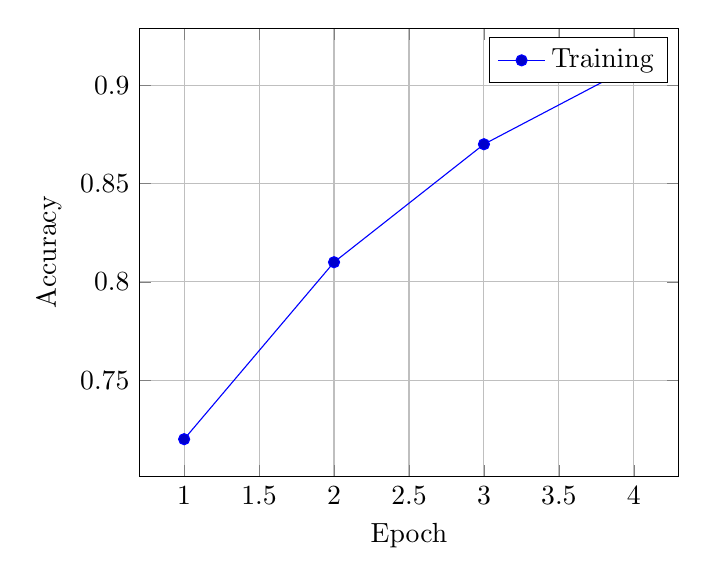
\begin{tikzpicture}
    \begin{axis}[xlabel=Epoch, ylabel=Accuracy, grid=both]
      \addplot coordinates {(1,0.72) (2,0.81) (3,0.87) (4,0.91)};
      \addlegendentry{Training}
    \end{axis}
  \end{tikzpicture}
  \caption{Training accuracy over epochs.}
  \label{fig:tikz-example}
\end{figure}
\end{verbatim}

\paragraph{Externalization.}
For large projects, enable figure caching to reduce compilation time:
\begin{verbatim}
\usetikzlibrary{external}
\tikzexternalize[prefix=tikz/]
\end{verbatim}

\section{Code Listings as Figures}

When code needs to be displayed, use the \texttt{listings} or \texttt{minted} package.  
Both can be styled to match \gls{novathesis} formatting.

\paragraph{Example using \texttt{listings}.}
\begin{verbatim}
\begin{figure}[h]
  \centering
  \begin{lstlisting}[language=Python,caption={Example Python script.},label={lst:python}]
  def add(a, b):
      return a + b
  \end{lstlisting}
\end{figure}
\end{verbatim}

\paragraph{Example using \texttt{minted}.}
\begin{verbatim}
\begin{listing}[h]
  \inputminted[fontsize=\small,frame=single]{python}{code/example.py}
  \caption{Example Python code.}
  \label{lst:minted}
\end{listing}
\end{verbatim}

When using \texttt{minted}, remember to compile with:
\begin{verbatim}
make xe LATEXMKOPTS="--shell-escape"
\end{verbatim}

\section{Captions and Descriptive Text}

\paragraph{Best practices.}
\begin{itemize}
  \item Every figure and table must include a descriptive caption.
  \item Captions should be concise, but self-contained.
  \item Avoid using abbreviations that are not defined in the text.
  \item Place figure captions \emph{below} figures and table captions \emph{above} tables.
\end{itemize}

\paragraph{Font and spacing.}
Captions inherit typographic settings from \gls{novathesis} defaults.  
They can be adjusted in \texttt{0-Config/0\_memoir.tex}:
\begin{verbatim}
\captionnamefont{\bfseries}
\captiontitlefont{\small}
\setlength{\abovecaptionskip}{10pt}
\setlength{\belowcaptionskip}{10pt}
\end{verbatim}

\section{Institutional Style Compliance}

Many institutions prescribe specific rules for figure and table formatting, including caption alignment, numbering, or placement.  
\gls{novathesis} allows these parameters to be tuned through configuration files:

\begin{itemize}
  \item Caption language and numbering are controlled by \texttt{mainlanguage} in \texttt{1\_novathesis.tex};
  \item Caption format and justification can be changed in \texttt{0-Config/0\_memoir.tex};
  \item List generation (Figures/Tables) is controlled via \texttt{0-Config/6\_list\_of.tex};
  \item Institutional color consistency should follow \texttt{style/colors} in \texttt{1\_novathesis.tex}.
\end{itemize}

Before submission, verify compliance with your institution’s thesis guidelines or formatting manual.

\section{Troubleshooting Common Float Issues}

\paragraph{Figure or table appears in the wrong place.}
This is normal in \LaTeX{}; floats move automatically.  
Add the option \texttt{[H]} from the \texttt{float} package to enforce fixed placement, but use sparingly.

\paragraph{Figures extend beyond margins.}
Reduce \texttt{width} or use \verb|\resizebox{\textwidth}{!}{...}|.

\paragraph{List of Figures or Tables missing.}
Ensure they are declared in \texttt{0-Config/6\_list\_of.tex} and that each figure or table includes a caption.

\paragraph{Subfigures misaligned.}
Ensure consistent \texttt{width} assignments and include \texttt{\textbackslash centering} inside each subfigure.

\section{Summary}

The \gls{novathesis} float system, based on the \texttt{memoir} class, provides a robust and consistent framework for managing figures, tables, and other visual elements.  
By following the conventions and configuration mechanisms described in this chapter, users can ensure clear, professional, and institution-compliant presentation of all illustrative material in their theses.

